\documentclass[a4paper,11pt]{book}
%\documentclass[a4paper,twoside,11pt,titlepage]{book}
\usepackage{listings}
\usepackage[utf8]{inputenc}
\usepackage{url}
\usepackage[spanish,es-tabla]{babel}

\usepackage{amsmath}
\usepackage{array}
\usepackage{booktabs}
\usepackage{tabulary}
\usepackage{multirow}

\usepackage{algorithm}
\usepackage[noend]{algpseudocode}

\makeatletter
\def\BState{\State\hskip-\ALG@thistlm}
\makeatother

% \usepackage[style=list, number=none]{glossary} %
%\usepackage{titlesec}
%\usepackage{pailatino}

\decimalpoint
\usepackage{dcolumn}
\newcolumntype{.}{D{.}{\esperiod}{-1}}
\makeatletter
\addto\shorthandsspanish{\let\esperiod\es@period@code}
\makeatother


%\usepackage[chapter]{algorithm}
\RequirePackage{verbatim}
%\RequirePackage[Glenn]{fncychap}
\usepackage{fancyhdr}
\usepackage{graphicx}
\usepackage{afterpage}

\usepackage{longtable}

\usepackage[pdfborder={0 0 0}]{hyperref}

% ********************************************************************
% Re-usable information
% ********************************************************************
\newcommand{\myTitle}{Nuevas propuestas de técnicas de recomendación para grupos\xspace}
\newcommand{\myMaster}{Máster en Ciencia de Datos e Ingeniería de Computadores\xspace}
\newcommand{\myName}{Juan José Sierra González\xspace}
\newcommand{\myProf}{Juan Manuel Fernández Luna\xspace}
\newcommand{\myFaculty}{Escuela Técnica Superior de Ingenierías Informática y de
Telecomunicación\xspace}
\newcommand{\myFacultyShort}{E.T.S. de Ingenierías Informática y de
Telecomunicación\xspace}
\newcommand{\myDepartment}{Departamento de Ciencias de la Computación e Inteligencia Artificial\xspace}
\newcommand{\myUni}{\protect{Universidad de Granada}\xspace}
\newcommand{\myLocation}{Granada\xspace}
\newcommand{\myTime}{\today\xspace}
\newcommand{\myVersion}{Version 0.1\xspace}


\hypersetup{
pdfauthor = {\myName (email (en) ugr (punto) es)},
pdftitle = {\myTitle},
pdfsubject = {},
pdfkeywords = {palabra\_clave1, palabra\_clave2, palabra\_clave3, ...},
pdfcreator = {LaTeX con el paquete ....},
pdfproducer = {pdflatex}
}

%\hyphenation{}


%\usepackage{doxygen/doxygen}
%\usepackage{pdfpages}
\usepackage{url}
\usepackage{colortbl,longtable}
\usepackage[stable]{footmisc}
%\usepackage{index}

%\makeindex
%\usepackage[style=long, cols=2,border=plain,toc=true,number=none]{glossary}
% \makeglossary

% Definición de comandos que me son tiles:
%\renewcommand{\indexname}{Índice alfabético}
%\renewcommand{\glossaryname}{Glosario}

\pagestyle{fancy}
\fancyhf{}
\fancyhead[LO]{\leftmark}
\fancyhead[RE]{\rightmark}
\fancyhead[RO,LE]{\textbf{\thepage}}
\renewcommand{\chaptermark}[1]{\markboth{\textbf{#1}}{}}
\renewcommand{\sectionmark}[1]{\markright{\textbf{\thesection. #1}}}

\setlength{\headheight}{1.5\headheight}

\newcommand{\HRule}{\rule{\linewidth}{0.5mm}}
%Definimos los tipos teorema, ejemplo y definición podremos usar estos tipos
%simplemente poniendo \begin{teorema} \end{teorema} ...
\newtheorem{teorema}{Teorema}[chapter]
\newtheorem{ejemplo}{Ejemplo}[chapter]
\newtheorem{definicion}{Definición}[chapter]

\definecolor{gray97}{gray}{.97}
\definecolor{gray75}{gray}{.75}
\definecolor{gray45}{gray}{.45}
\definecolor{gray30}{gray}{.94}

\lstset{ frame=Ltb,
     framerule=0.5pt,
     aboveskip=0.5cm,
     framextopmargin=3pt,
     framexbottommargin=3pt,
     framexleftmargin=0.1cm,
     framesep=0pt,
     rulesep=.4pt,
     backgroundcolor=\color{gray97},
     rulesepcolor=\color{black},
     %
     stringstyle=\ttfamily,
     showstringspaces = false,
     basicstyle=\scriptsize\ttfamily,
     commentstyle=\color{gray45},
     keywordstyle=\bfseries,
     %
     numbers=left,
     numbersep=6pt,
     numberstyle=\tiny,
     numberfirstline = false,
     breaklines=true,
   }
 
% minimizar fragmentado de listados
\lstnewenvironment{listing}[1][]
   {\lstset{#1}\pagebreak[0]}{\pagebreak[0]}

\lstdefinestyle{CodigoC}
   {
	basicstyle=\scriptsize,
	frame=single,
	language=C,
	numbers=left
   }
\lstdefinestyle{CodigoC++}
   {
	basicstyle=\small,
	frame=single,
	backgroundcolor=\color{gray30},
	language=C++,
	numbers=left
   }

 
\lstdefinestyle{Consola}
   {basicstyle=\scriptsize\bf\ttfamily,
    backgroundcolor=\color{gray30},
    frame=single,
    numbers=none
   }


\newcommand{\bigrule}{\titlerule[0.5mm]}


%Para conseguir que en las páginas en blanco no ponga cabecerass
\makeatletter
\def\clearpage{%
  \ifvmode
    \ifnum \@dbltopnum =\m@ne
      \ifdim \pagetotal <\topskip
        \hbox{}
      \fi
    \fi
  \fi
  \newpage
  \thispagestyle{empty}
  \write\m@ne{}
  \vbox{}
  \penalty -\@Mi
}
\makeatother

\usepackage{pdfpages}
\begin{document}
\begin{titlepage}
 
 
\newlength{\centeroffset}
\setlength{\centeroffset}{-0.5\oddsidemargin}
\addtolength{\centeroffset}{0.5\evensidemargin}
\thispagestyle{empty}

\noindent\hspace*{\centeroffset}\begin{minipage}{\textwidth}

\centering

\includegraphics[width=0.9\textwidth]{imagenes/logo_ugr.jpg}\\[1.4cm]

\textsc{ \Large TRABAJO FIN DE MÁSTER\\[0.2cm]}
\textsc{MÁSTER UNIVERSITARIO OFICIAL EN CIENCIA DE DATOS E INGENIERÍA DE COMPUTADORES}\\[1cm]
% Upper part of the page
% 
% Title
{\Huge\bfseries Nuevas propuestas de técnicas de recomendación para grupos\\
}
\noindent\rule[-1ex]{\textwidth}{2pt}\\[3.5ex]
%{\large\bfseries Implementación, estudio y comparativa}
\end{minipage}

\vspace{2cm}
\noindent\hspace*{\centeroffset}\begin{minipage}{\textwidth}
\centering

\textbf{Autor}\\ {Juan José Sierra González}\\[2.5ex]
\textbf{Tutor}\\
{Juan Manuel Fernández Luna}\\[2cm]

\includegraphics[width=0.3\textwidth]{imagenes/etsiit_logo.png}\\[0.1cm]
\textsc{Escuela Técnica Superior de Ingenierías Informática y de Telecomunicación}\\
\textsc{---}\\
Granada, enero de 2020
\end{minipage}
%\addtolength{\textwidth}{\centeroffset}
%\vspace{\stretch{2}}
\end{titlepage}



\chapter*{}
%\thispagestyle{empty}
%\cleardoublepage

%\thispagestyle{empty}

\begin{titlepage}
 
 
\setlength{\centeroffset}{-0.5\oddsidemargin}
\addtolength{\centeroffset}{0.5\evensidemargin}
\thispagestyle{empty}

\noindent\hspace*{\centeroffset}\begin{minipage}{\textwidth}

\centering
%
\includegraphics[width=0.9\textwidth]{imagenes/logo_ugr.jpg}\\[1.4cm]

%\textsc{ \Large PROYECTO FIN DE CARRERA\\[0.2cm]}
%\textsc{ INGENIERÍA EN INFORMÁTICA}\\[1cm]
% Upper part of the page
% 

 \vspace{3.3cm}

%si el proyecto tiene logo poner aquí
 \vspace{0.5cm}

% Title

{\Huge\bfseries Nuevas propuestas de técnicas socioinspiradas de recomendación para grupos\\
}
\noindent\rule[-1ex]{\textwidth}{2pt}\\[3.5ex]
%{\large\bfseries Implementación, estudio y comparativa\\[4cm]}
\end{minipage}

\vspace{2.5cm}
\noindent\hspace*{\centeroffset}\begin{minipage}{\textwidth}
\centering

\textbf{Autor}\\ {Juan José Sierra González}\\[2.5ex]
\textbf{Tutor}\\
{Juan Manuel Fernández Luna}\\[2cm]
%\includegraphics[width=0.15\textwidth]{imagenes/tstc.png}\\[0.1cm]
%\textsc{Departamento de Teoría de la Señal, Telemática y Comunicaciones}\\
%\textsc{---}\\
%Granada, mes de 201
\end{minipage}
%\addtolength{\textwidth}{\centeroffset}
\vspace{\stretch{2}}

 
\end{titlepage}






\cleardoublepage
\thispagestyle{empty}

\begin{center}
{\large\bfseries Sistemas de recomendación de películas para grupos}\\
\end{center}
\begin{center}
Juan José Sierra González\\
\end{center}

%\vspace{0.7cm}
\noindent{\textbf{Palabras clave}: incluir palabras clave...}\\

\vspace{0.7cm}
\noindent{\textbf{Resumen}}\\

Incluir resumen...
\cleardoublepage


\thispagestyle{empty}


\begin{center}
{\large\bfseries Group recommender systems for movies}\\
\end{center}
\begin{center}
Juan José Sierra González\\
\end{center}

%\vspace{0.7cm}
\noindent{\textbf{Keywords}: include keywords...}\\

\vspace{0.7cm}
\noindent{\textbf{Abstract}}\\

Include abstract...

\chapter*{}
\thispagestyle{empty}

\noindent\rule[-1ex]{\textwidth}{2pt}\\[4.5ex]

Yo, \textbf{Juan José Sierra González}, alumno del Máster Universitario Oficial en Ciencia de Datos e Ingeniería de Computadores de la \textbf{Escuela Técnica Superior de Ingenierías Informática y de Telecomunicación de la Universidad de Granada}, con DNI 76589592Y, autorizo la
ubicación de la siguiente copia de mi Trabajo Fin de Máster en la biblioteca del centro para que pueda ser
consultada por las personas que lo deseen.

\vspace{6cm}

\noindent Fdo: Juan José Sierra González

\vspace{2cm}

\begin{flushright}
Granada a 9 de enero de 2020.
\end{flushright}


\chapter*{}
\thispagestyle{empty}

\noindent\rule[-1ex]{\textwidth}{2pt}\\[4.5ex]

D. \textbf{Juan Manuel Fernández Luna}, Profesor del Área de Uncertainty Treatment in Artificial Intelligence del Departamento de Ciencias de la Computación e Inteligencia Artificial de la Universidad de Granada.

\vspace{0.5cm}

\textbf{Informa:}

\vspace{0.5cm}

Que el presente trabajo, titulado \textit{\textbf{Sistemas de recomendación de películas a grupos}},
ha sido realizado bajo su supervisión por \textbf{Juan José Sierra González}, y autoriza la defensa de dicho trabajo ante el tribunal
que corresponda.

\vspace{0.5cm}

Y para que conste, expide y firma el presente informe en Granada a 9 de enero de 2020.

\vspace{1cm}

\textbf{El director:}

\vspace{5cm}

\noindent \textbf{Juan Manuel Fernández Luna}

\chapter*{Agradecimientos}
\thispagestyle{empty}

\vspace{1cm}

Incluir agradecimientos...
\frontmatter
\tableofcontents
\listoffigures
\listoftables

\mainmatter
\setlength{\parskip}{5pt}

\chapter{Introducción}



\section{Motivación}



\section{Objetivos}


\chapter{Planificación}

En este capítulo se aborda el plan de trabajo a seguir para la realización de este estudio. En primar lugar se realizará la captación de requisitos necesarios para lograr el objetivo propuesto, y después se detallará la planificación del trabajo, con una estimación en costes tanto de trabajo como de materiales así como una distribución del tiempo entre tareas.

Al tratarse de un trabajo de investigación, no se puede realizar adecuadamente el análisis de requisitos habitual para un proyecto general de ingeniería. En su lugar, sin embargo, se plantean unas etapas diferentes que se deben cumplir para llevar a cabo un estudio de estas características.

\section{Etapas de investigación}

Las etapas del proceso de investigación de este estudio son las siguientes:

\begin{enumerate}
	\item{\textbf{Realizar una investigación inicial en torno a los sistemas de recomendación}: revisar la literatura buscando información acerca de estos sistemas, comprobar qué evolución han seguido a lo largo de los años y cómo se han llegado a desarrollar los sistemas de recomendación a grupos.}
	\item{\textbf{Profundizar en el estado del arte del sistemas de recomendación a grupos}: investigar más a fondo en estos métodos que son en los que realmente se va a centrar el estudio. Obtener los sistemas más destacados del estado del arte.}
	\item{\textbf{Seleccionar el algoritmo de referencia del estado del arte}: Entre todos los sistemas de recomendación a grupos que se hayan investigado en el paso anterior, decidir cuál es el que se ajusta mejor a los requerimientos del estudio y obtener toda la información necesaria para implementarlo.}
	\item{\textbf{Crear los grupos para el experimento}: decidir qué métodos se van a seguir para la división de usuarios en grupos y crearlos desde el primer momento de la experimentación para así trabajar siempre sobre los mismos.}
	\item{\textbf{Implementar las estrategias de combinación}: seleccionar qué estrategias se van a utilizar en el estudio para combinar las valoraciones individuales de los miembros del grupo y así obtener una valoración grupal.}
	\item{\textbf{Implementar el algoritmo del estado del arte}: implementar el método siguiendo los parámetros y estructura del experimento diseñado. Es necesario contar con el código de los algoritmos para el experimento, por lo que hay que implementar el del estado del arte si no se puede conseguir su código fuente.}
	\item{\textbf{Diseñar las nuevas propuestas del estudio}: para el objetivo del estudio hay que plantear nuevas propuestas que puedan competir con el estado del arte. Para ello primero hay que valorar los campos que quedan por experimentar y proponer una serie de algoritmos que se ajusten al perfil buscado.}
	\item{\textbf{Implementar las propuestas propias}: una vez decididas las propuestas que van a formar parte del experimento, se deben implementar del mismo modo que el algoritmo del estado del arte. Comprobar de nuevo que toda la funcionalidad del experimento es válida con la nueva implementación.}
	\item{\textbf{Diseñar la evaluación de los modelos}: se debe decidir qué métrica de evaluación se va a utilizar, e implementar un algoritmo \textit{baseline} que sirva como punto de referencia base.} 
	\item{\textbf{Obtener los resultados del experimento}: obtener a través de la implementación del experimento los resultados del mismo. Se pueden visualizar los datos con tablas y gráficos que sean adecuados para el estudio.}
	\item{\textbf{Realizar un análisis de los resultados obtenidos}: comparar los resultados de cada método con el método de referencia \textit{baseline} y con el método del estado del arte, así como entre ellos, a fin de descubrir qué algoritmo se comporta mejor para cada caso, tanto entre grupos formados de distinta forma como con estrategias de agregación diferentes.}
	\item{\textbf{Extraer conclusiones del estudio realizado}: dar una visión analítica de la eficacia de las propuestas ideadas para el estudio, apoyándose en los resultados obtenidos con respecto a los algoritmos de referencia, y justificar cuáles de ellas son más prometedoras.}
	\item{\textbf{Considerar trabajos futuros a realizar}: valorar en qué aspectos se puede seguir progresando en los métodos propuestos en el estudio, así como proponer nuevas tareas o retos dentro de este ámbito de investigación que no se hayan abarcado en el proceso del mismo.}
\end{enumerate}

Con las diferentes etapas planteados, la planificación del trabajo debe ocupar los pasos que se han definido y estimar un tiempo con el que se podría solventar cada una. Además, debe describir todo el material e infraestructura necesarios y, junto al tiempo estimado, dar una idea del presupuesto que requiere realizar este estudio.

\section{Planificación del trabajo}

Este apartado está subdividido en estimación de costes y estimación de tiempo. En un primer lugar se valora el coste de la infraestructura utilizada, así como de todo el material que se haya utilizado y que esté disponible de forma libre y gratuita. A partir de ahí se puede realizar un presupuesto base del que partir. La estimación de tiempo debe ser realista y que permita cumplir los requisitos en un plazo competente, a fin de no necesitar aplazar los tiempos a última hora debido a una mala planificación. De ser así habría que cargar con el consecuente aumento en costes.

\subsection{Estimación de coste de materiales e infraestructura}

En primer lugar se tendrá en cuenta el ordenador con la que se ha desarrollado este estudio. Se trata de un ordenador portátil de la marca MSI, del año 2019, y que cuenta con un procesador i7-8750H capaz de llegar a 4.1GHz, así como con 16GB de memoria RAM DDR4-2666, una gráfica GeForce GTX 1060 6GB GDDR5 y dos SSD de 512GB cada uno, uno de los cuales tiene un SO Windows y el otro un SO Linux. Con este equipo se han realizado todas las tareas de investigación, implementación y evaluación: documentación, revisión de la literatura y redacción de la memoria, labores de desarrollo e implementación de los algoritmos y ejecución del experimento para obtención de resultados.

Para obtener la información y documentación requerida para el trabajo ha sido necesaria una red de internet de banda ancha, disponible tanto en el lugar de desarrollo del trabajo como en las instalaciones de la Universidad de Granada cuando ha sido necesario. Gracias a los convenios que la Universidad establece con algunas bases de datos documentales como Scopus \cite{scopus-website} ha sido posible acceder a multitud de \textit{papers} y publicaciones sobre el tema a investigar. Además ha sido de mucha utilidad la página ResearchGate \cite{research-gate-website} para acceder a otros papers no encontrados en Scopus.

El desarrollo del trabajo ha sido realizado completamente sobre el sistema operativo Linux, con una distribución Pop\_OS! \cite{pop-os} basada en Ubuntu 18.10, por lo que es totalmente libre y carente de costes. Las principales herramientas de software utilizadas también han sido de código abierto por lo que no han conllevado coste adicional, utilizando como IDE principal para el desarrollo Visual Studio Code \cite{vscode-github} y escribiendo la memoria en LaTeX utilizando el software TeXstudio \cite{texstudio}, disponible para Ubuntu. 

El proyecto ha sido libre desde el primer momento, siendo alojado en la plataforma \textbf{GitHub} \cite{github-proyecto}. Allí se puede comprobar los pasos que se han seguido durante la implementación, así como observar cómo se ha diseñado, desarrollado y evolucionado el proyecto con el paso del tiempo. Cualquier usuario puede acceder al código de forma totalmente gratuita, así como trabajar sobre él realizando los cambios que considere, cumpliendo el paradigma del software libre.

De todo este material expuesto en los párrafos anteriores, el trabajo sólo ha requerido comprar el ordenador portátil personal y la red de banda ancha disponible en el lugar de desarrollo del mismo, dado que se trata de recursos personales. El resto de la infraestructura y materiales o bien han sido productos de software libre o han sido aportados por la Universidad de Granada.

\subsection{Distribución temporal de las tareas}

Organizar la carga de trabajo en las distintas fases del estudio es una labor que debe plantearse previo a la realización del mismo. Con el planteamiento correctamente definido se pueden decidir algunas fechas de entrega y acotar los tiempos que se le asignan a cada tarea. Gracias a ello, el progreso del proyecto puede seguir el curso planificado, es más sencillo modularizar las tareas y así finalizar en el tiempo estimado.

En primer lugar, la labor de revisión de la literatura ocupará los primeros pasos del trabajo. El estudio debe partir de un punto en el que se conozcan correctamente los detalles de los sistemas de recomendación, con todas sus características. Por supuesto, debe haberse hecho una búsqueda de documentos que tengan dicha información, así como de aquellos \textit{papers} que contengan planteamientos de algoritmos de interés. Se seleccionan las propuestas más interesantes a priori, una vez se ha investigado lo suficiente sobre el tema y se han recabado suficientes ejemplos. La realización de esta tarea puede llevar un mes.

La documentación debe ser un proceso que se lleve de principio a fin, de manera que se vayan tomando notas y documentando adecuadamente conforme se va obteniendo la información requerida. No se puede poner una estimación a priori debido a su carácter cambiante y adaptativo en función del progreso del propio trabajo.

En cuanto al diseño del experimento, es una tarea compleja que lleva una carga de trabajo considerable. Montar todo el entorno, elegir qué estructuras de datos se van a utilizar, cómo automatizar los procesos y cómo almacenar los resultados obtenidos requiere tomar una serie de decisiones cruciales a la hora de definir el proyecto. Cometer un error en este punto supone más tiempo de corrección conforme más avance se haya realizado en el experimento, por lo que es una labor puntillosa a la que merece la pena dedicar tiempo. Al menos se plantean dos semanas o un mes de plazo para terminar toda esta estructura.

Para la implementación del sistema de recomendación del estado del arte de acuerdo al entorno experimental que se haya montado puede requerir un poco de tiempo, pero al fin y al cabo el algoritmo está definido y no debería suponer más de dos semanas seguir los pasos indicados en la publicación. En algunos casos puede haber determinadas partes que no estén bien especificadas y requiera o bien más labor de investigación o bien tomar alguna decisión propia sobre la implementación (propiamente documentada en su correspondiente apartado).

Con respecto a las nuevos métodos de recomendación para el estudio, cabe destacar que no requiere únicamente labor de implementación sino que también hay que detenerse a analizar el estado del arte y pensar en qué vertientes pueden aportarse al ámbito tratado. Aunque la mayor parte de esta tarea se pueda hacer en el apartado de revisión de la literatura, es en este punto, ya habiendo implementado el algoritmo actual, cuando es más sencillo darse cuenta de aquello que se ha echado en falta durante la investigación e implementación. Como además no se ha limitado desde el primer momento el número de nuevas propuestas que puedan surgir, se ha planteado dejar un mes para todo el proceso de análisis e implementación de dichas propuestas.

Para la ejecución del experimento y la obtención de datos se pueden utilizar un par de días o incluso una semana, a fin de recopilar en tablas los valores obtenidos y conseguir visualizar los datos de manera óptima para que reflejen los objetivos deseados. De esta forma se podrá comprobar de un vistazo sencillo el impacto de cada sistema de recomendación frente al problema planteado en cada caso.

Finalmente, extraer conclusiones de los resultados puede ser más sencillo si se conocen los algoritmos y se han trabajado correctamente, de forma que sea fácil interpretarlos y descubrir patrones en los mismos. Al ser una tarea tan diversa y poco acotada, una extracción de conclusiones puede llevar desde unos días hasta una semana.

En resumen, este trabajo de investigación puede enmarcarse en el tiempo en unos 4 meses, aunque naturalmente esa estimación puede variar en función del tiempo que se le pueda dedicar diariamente al proyecto, especialmente si se compagina con un trabajo a jornada completa. Es de importancia recordar que el tiempo invertido en el experimento también tiene un coste, igual que el de los materiales e infraestructura; en esencia se trata de otro recurso. Partiendo de la base de que este estudio es un trabajo de investigación en un campo puntero tecnológicamente, podría estimarse el coste total del trabajo como una media entre el sueldo a jornada completa de un ingeniero informático junior y el de un investigador de un departamento de universidad durante el transcurso del mismo.

Estimando para una profesión de estas características un valor aproximado de 12 euros/hora, a 4 meses trabajando (20 días al mes) y dedicándole una media de 4h diarias, se estipularía el presupuesto del proyecto en 2880 euros.

A continuación se ilustra el proceso con un cronograma generado gracias a la plataforma libre \textit{draw.io} \cite{draw.io}:

\begin{figure}[H]
	\centering
	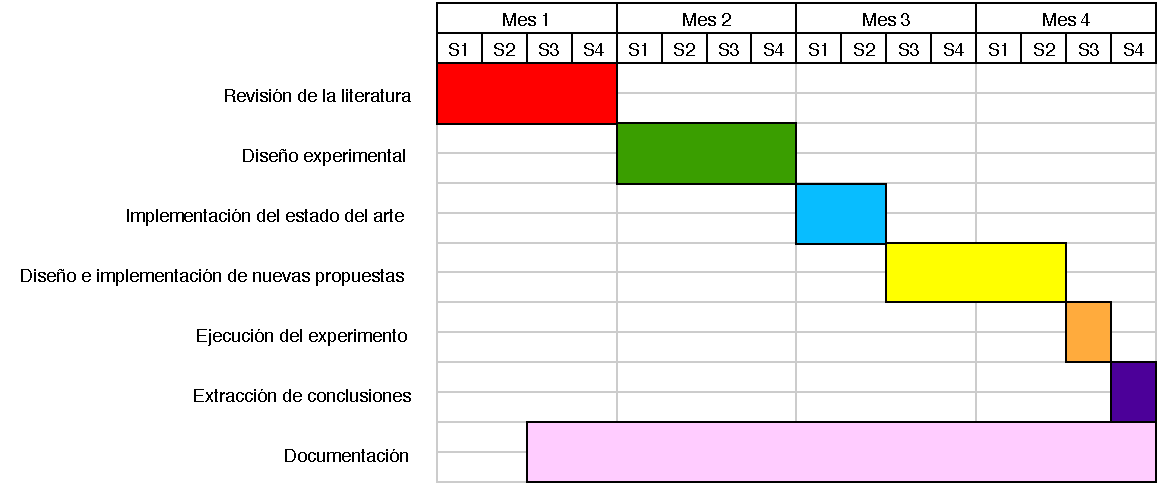
\includegraphics[scale=0.6]{imagenes/cronograma.pdf}
	\caption{Cronograma ilustrativo de la planificación del estudio.}
	\label{cronograma}
\end{figure}
\chapter{Revisión de la literatura: estado del arte}

En este capítulo se expondrá una revisión de los estudios y propuestas más innovadoras relacionadas con los \textbf{sistemas de recomendación a grupos}, y en particular, de aquellos orientados al ámbito de las películas. Se comenzará haciendo un breve inciso sobre cuándo y cómo se originaron los sistemas de recomendación, así como la particularidad de aquellos específicos de recomendación a grupos. Después se tratará su evolución hasta nuestros días, realizando un comentario analítico acerca de lo que han supuesto los sistemas de recomendación y cómo se trasladan actualmente dichos sistemas a situaciones cotidianas, con algunos claros ejemplos que todo el mundo utiliza. Entre ellos se destacarán los que abarcan la \textbf{recomendación de películas}, como tema principal del estudio. Por último, se mencionarán algunos de los sistemas de recomendación de películas a grupos más actuales, eligiendo además el que será tomado como referencia para la experimentación como representante del estado del arte de estos recomendadores.

Queda ya muy atrás el primer sistema de recomendación de la historia, que vio la luz en 1992, cuando Goldberg et al. (1992) presentaron su artículo \textit{``Using collaborative filtering to Weave an Information tapestry''} \cite{tapestry-goldberg}. En este trabajo se acuña por primera vez el término \textbf{``filtrado colaborativo''} (en inglés, \textit{collaborative filtering}), refiriéndose así a la técnica que permite filtrar elementos a un usuario basándose en lo que otros usuarios han opinado de él anteriormente. Esta técnica sienta las bases de los sistemas de recomendación, y aún a día de hoy se encuentra presente en la mayoría de ellos. La otra alternativa al filtrado colaborativo es el \textbf{filtrado basado en contenido} (en inglés, \textit{content-based filtering}). Esta técnica no tiene en cuenta las valoraciones que otros usuarios han dado a los elementos del sistema, sino que se limita a comparar los elementos por características y recomendar aquellos similares. En este experimento, sin embargo, se tratarán únicamente métodos que utilizan el filtrado colaborativo.

Una vez se hubo contemplado el vasto rango de opciones que albergaban los sistemas de recomendación, a través de numerosos trabajos y estudios, se contempló la posibilidad de recomendar ya no solo a individuos, sino a grupos de personas. Se trataba de una situación a la que una sociedad podía enfrentarse en multitud de facetas, y que sin duda merecía la pena explorar. La pionera, y una de las más famosas y reconocidas propuestas sobre este tema, fue \textbf{PolyLens} \cite{polylens}. En esta publicación de 2001, O'Connor et al. plantearon \textbf{un sistema de recomendación de películas para grupos}, derivado de la base de datos de valoraciones de películas \textbf{MovieLens}, en la que varios trabajos anteriores se habían fundado. Este sistema abrió la veda de un nuevo subgrupo dentro de la ya amplia categoría de sistemas de recomendación.

Como se ha comentado anteriormente, las recomendaciones a películas han levantado mucho interés desde el primer momento. El contenido de ocio audiovisual, junto a los catálogos de tiendas \textit{online}, son los casos de mayor demanda en cuanto a sistemas de recomendación en la sociedad actual. Plataformas como \textbf{Netflix}, \textbf{Spotify} o \textbf{HBO} son ejemplos de los primeros, que utilizan estos sistemas para tratar de mantener al usuario satisfecho ofreciéndole nuevo contenido que sea similar al que hayan visto. Por su parte, \textbf{Amazon} o \textbf{AliExpress} son ejemplos de los segundos, grandes plataformas que dan cabida a todo tipo de productos y que son capaces de recomendar a sus clientes otros productos similares a los que están buscando. Gracias al sistema de recomendación pertinente, incluso consiguen ofrecer nuevos artículos que detectan que el usuario puede querer comprar, basándose en lo que anteriormente ha buscado o comprado.

Tal fue el impacto de los sistemas de recomendación que la propia plataforma Netflix lanzó en 2006 lo que se conocería como el \textbf{Netflix Prize} \cite{netflix-prize}, una competición de sistemas que, basándose únicamente en el filtrado colaborativo (no conociendo datos adicionales sobre películas ni sobre usuarios, solamente las valoraciones que estos habían dado a cada película) fueran capaces de predecir acertadamente dichas valoraciones. El objetivo principal era superar al por aquel entonces actual sistema de recomendación de Netflix, conocido como \textbf{Cinematch}, ofreciendo un premio de 1 millón de dólares a aquel sistema capaz de superarlo en un 10\%. Adicionalmente, como la competición se estimaba que duraría hasta 2011, se concedería un premio anual de 50.000 dólares al método ganador al final de cada año.

Tras varios tira y afloja entre algunos equipos, e incluso agrupaciones entre equipos para forjar mejores ideas juntos, finalmente en 2009 el equipo \textit{'BellKor's Pragmatic Chaos'} se alzó ganador y recibió el gran premio \cite{netflix-prize-winner}, superando al algoritmo anterior por 10.05\%. De esta forma tan original Netflix cambió su sistema de recomendación promoviendo una iniciativa de investigación en este campo, y por supuesto previendo que este avance en su algoritmo les serviría para incrementar la satisfacción de sus clientes, y por ende, para aumentar su valor de mercado.

Tras haber sido puestos en el panorama de investigación con casos como el Netflix Prize y el evidente aumento de su uso conforme las nuevas tecnologías se han vuelto más accesibles para la sociedad, los sistemas de recomendación han contemplado un gran abanico de variedades: algunos más enfocados a la materia que recomendar (por ejemplo, sistemas de recomendación de música o de películas), otros enfocados al tipo de usuario (sistemas de recomendación individual o a grupos) e incluso algunos cuyo propósito no es solamente obtener el mejor resultado (sistemas de recomendación explicativos que sirvan de apoyo a una decisión).

Como el objetivo de este trabajo es orientarse en recomendación a películas para grupos de usuarios, la búsqueda en la literatura de algoritmos que apoyasen el estudio se focalizó en estos dos grandes campos, analizando algunos algoritmos de la última década. La recomendación a grupos ha avanzado a muchos niveles desde la presentación de PolyLens, y ahora existen varios frentes abiertos en investigación sobre este tema.

Uno de las primeras fuentes que se recopilaron sobre los sistemas de recomendación a grupos, y que han servido a este estudio para obtener información general sobre los mismos, es el capítulo de Masthoff en el \textit{Recommender Systems Handbook} de 2011 \cite{masthoff-handbook}, donde hace un repaso a los campos de investigación abiertos de los que se hablaba en el párrafo anterior, y realiza un análisis sobre los pasos a seguir en adelante. Masthoff sienta en primer lugar los motivos por los que es necesario contar con sistemas de recomendación a grupos frente a la recomendación individual que ya se había trabajado más de una década. Aporta una detallada recopilación de las estrategias de agregación que utilizaban los sistemas de recomendación a grupos más interesantes de la época, como el ya mencionado PolyLens \cite{polylens}, el sistema MusicFX \cite{musicfx} que determina la emisora de radio que suena de fondo en un gimnasio en función de los gustos de la gente que haya ejercitándose en ese momento, o el sistema Intrigue \cite{intrigue} que ayuda a grupos de turistas a decidir qué visitar, entre otros. A continuación explica cómo se pueden aplicar los algoritmos de recomendación a grupos para usuarios individuales, dando a entender que estos algoritmos son reutilizables dependiendo del contexto en el que se necesiten. Termina planteando una serie de retos a los que los sistemas de recomendación a grupos se enfrentaban en aquel momento: aportar explicaciones a las recomendaciones propuestas, profundizar en el ``problema del inicio frío'' para grupos de usuarios o recomendar ítems en un determinado orden.

En el contexto de las recomendaciones ordenadas podrían englobarse los \textbf{rankings}, que es hacia donde han evolucionado los recomendadores individuales en las principales páginas. Es habitual no limitarse a recomendar un único ítem a un usuario, lo que propicia que se investigue en recomendar series de elementos dándoles un determinado orden (por supuesto, se quiere colocar en primer lugar aquel que se prediga que va a tener más aceptación).
\chapter{Nuevas propuestas aportadas al estudio}

En este capítulo se realizará un análisis sobre los distintos métodos ideados para competir contra el sistema de recomendación del estado del arte que se ha escogido como referencia. La idea es proponer una serie de alternativas que puedan resultar interesantes y que se espera que mejoren la eficacia de dicho método.

Como se ha mencionado en el capítulo anterior, el principal criterio que se ha seguido para escoger el método del estado del arte es, aparte de la intrínseca necesidad de tratarse de un algoritmo actual, que reproduzca en su algoritmo un comportamiento social que se asemeje a la toma de decisiones que realizan los seres humanos a la hora de enfrentarse a un problema así. En el caso del sistema de recomendación de referencia, su algoritmo se basa en decidir qué usuario es más representativo para el grupo en función de la lista de preferencias que tiene cada miembro. Para los métodos propios de este estudio se han planteado las siguientes propuestas:

\begin{itemize}
	\item \textbf{Método de empatía}
	\item \textbf{Método del más cinéfilo}
	\item \textbf{Método del más optimista}
	\item \textbf{Método de mayor similitud}
\end{itemize}

A lo largo de las próximas páginas se realizará un análisis más detallado acerca de cada uno de estos métodos, así como de dónde ha surgido la idea de cada uno y cómo puede asemejarse a un comportamiento social. Además se explicará su funcionamiento mediante pseudocódigo acompañado de una descripción del mismo en lenguaje natural.

\section{Método de empatía}

La idea para esta primera propuesta surgió desde el inicio del estudio, ya que fue un factor que no se identificó en prácticamente ningún sistema de recomendación a grupos del estado del arte. En el recomendador \textit{HappyMovie} \cite{happymovie2011} aparecía el concepto de \textit{fairness}, algo así como la ``justicia'' a la hora de realizar recomendaciones al grupo. Sin embargo, en dicha publicación no se hace referencia al método que utilizan para medir, estimar y recalcular el valor de \textit{fairness} a lo largo del tiempo. Dada la naturaleza del concepto, este valor tiene necesariamente que ser dinámico y actualizarse en función de lo que haya ocurrido en iteraciones pasadas. En este punto se decidió que una de las nuevas propuestas del estudio fuera \textbf{un sistema de recomendación a grupos capaz de ser empático} con todos los miembros del mismo.

La premisa para este algoritmo es sencilla, pero lógica: dar más importancia a las preferencias de aquellos usuarios a los que menos les hayan gustado las últimas películas recomendadas. A un usuario al que no le hayan gustado nada las últimas tres películas recomendadas se le tendrá muy en cuenta a la hora de decidir la siguiente, de la misma manera que a una persona a la que le han maravillado esas mismas películas no le importará que la siguiente le guste un poco menos.

Si se habla de un grupo de amigos que van a ver una película, este algoritmo tiene especial sentido, ya que se entiende que todos los miembros buscan el interés general del grupo además de su propio beneficio. Estar dispuesto a hacer concesiones, o ``sacrificar'' una elección óptima para que otra parte del grupo obtenga una opción mejor hace que el grupo se equilibre y puede dar lugar a una recomendación interesante desde el punto de vista algorítmico -- a través de la experimentación se dictaminará si también lo es desde el punto de vista de la eficacia.

A continuación se muestra un fragmento de pseudocódigo que representa el método de recomendación basado en empatía:
\newpage

\begin{algorithm}
	\caption{Método de empatía}
	\begin{algorithmic}[1]
		\State $valoraciones \gets predecirValoraciones()$
		\For{\textit{usuario} \textbf{in} \textit{grupo}}
		\State \textbf{Añadir} $\frac{1}{size(grupo)}$ \textbf{a} \textit{pesos}
		\EndFor
		\State $ranking \gets []$
		\While{\textit{size(películas)} \textbf{$> 1$}}
		\State $valoracionesPonderadas \gets valoraciones \times pesos$
		\State \textit{películaRecomendada} $ \gets max(valoracionesPonderadas)$
		\State $pesos \gets actualizarPesos()$
		\State \textbf{Eliminar} \textit{películaRecomendada} \textbf{de} \textit{valoraciones} \textbf{y} \textit{películas}
		\State \textbf{Añadir} \textit{películaRecomendada} \textbf{a} \textit{ranking}
		\EndWhile
		\State \textbf{Añadir última} \textit{película} \textbf{a} \textit{ranking}
		\State{\textbf{return} \textit{ranking}}
	\end{algorithmic}
\end{algorithm}

\begin{algorithm}
	\caption{Actualización de pesos para el método de empatía}
	\begin{algorithmic}[1]
		\State \textit{rango} $\gets 0.2$
		\State \textit{paso} $\gets \frac{rango}{size(grupo) - 1}$
		\State \textit{ordenSatisfacción} $\gets$ \textbf{Ordenar} \textit{valoraciones[películaRecomendada]}
		\For{\textit{posición} \textbf{in} \textit{ordenSatisfacción}}
		\State \textit{pesos[posición]} $\gets -\frac{rango}{2} + paso \times $\textit{posición}
		\EndFor
		\State \textbf{return} \textit{pesos}
	\end{algorithmic}
\end{algorithm}

En el pseudocódigo se pueden observar dos algoritmos distinguidos: el primero representa el grueso del método, con todo el proceso del sistema de recomendación y que devuelve el ranking final; el segundo es el algoritmo que actualiza los pesos para cada miembro del grupo en función de cuánto les ha gustado la película. En las siguientes líneas se entenderán qué son estos pesos y cómo afectan al criterio de selección diseñado.

En primer lugar, se analizará el algoritmo general del sistema de recomendación. Este método tiene una clara diferencia que destaca sobre el algoritmo del estado del arte, y es la presencia de \textbf{pesos} que ponderan la relevancia de cada miembro del grupo, entendiendo por relevancia lo mucho que puede influir un miembro en la toma de una decisión determinada en el transcurso de la construcción del ranking final. Es decir, estos pesos tienen que ser \textbf{dinámicos} para adaptarse a las circunstancias que se vayan aprendiendo de las iteraciones anteriores.

La inicialización de valores que se da al comienzo del algoritmo conlleva la creación de un vector de pesos que, por el momento, debe valorar a todos los usuarios por igual. Se entiende que se parte desde un punto base en el que ningún usuario está más satisfecho que otro, por lo tanto todos tienen la misma importancia a la hora de tomar una decisión sobre qué película deben escoger. Para lograr esta funcionalidad, a cada usuario de un grupo $G$ debe serle asignado un valor equivalente a $\frac{1}{|G|}$, siendo $|G|$ la cardinalidad de dicho grupo, y así conseguir que todos aporten el mismo porcentaje a la decisión final.

Para poder comenzar a recomendar cualquier película a un grupo, es necesario que se cuente con una estimación de lo que cada miembro va a valorar dicha película. Esto se consigue mediante \textbf{predicción} -- el método utilizado para ello se explicará en detalle en el apartado correspondiente a experimentación, dado que se puede sustituir fácilmente en función del estudio que se quiera realizar, y qué algoritmo se elija para predecir estas valoraciones no implica cambio alguno en cuanto a cómo se desarrolla el método.

Con la matriz de valoraciones obtenida (películas x miembros del grupo) y los pesos inicializados, se comienza un bucle del que obtener en cada iteración la película seleccionada para ser incluida en el ranking. Para ello, lo primero que hay que hacer es computar los pesos para cada usuario, dándoles a la valoración de cada uno un coeficiente de modificación que se corresponda a la importancia que han de tener en la decisión pertinente. Una vez obtenidas las valoraciones ponderadas, sumando dichas valoraciones para cada película se calcula cuál obtiene un resultado mayor, y por tanto \textbf{es la película recomendada}. El último paso de este bucle es añadir la película al ranking final (por supuesto, ordenado), eliminarla de la lista de películas y de la matriz de valoraciones, y \textbf{recalcular los pesos} asignados a cada usuario.

Al tratarse de un método un poco más complejo, se ha decidido separar este algoritmo del pseudocódigo del sistema de recomendación, y en cierto modo también realizar un paréntesis en la explicación del mismo para analizar cómo se actualizan los pesos de los usuarios en este método en particular. Como se ha indicado anteriormente, la funcionalidad principal que se persigue con este método es que los usuarios queden \textbf{satisfechos de forma empática}, es decir, se busca propiciar que los usuarios que no han visto películas que les gustan tengan más voz a la hora de escoger la siguiente. En este algoritmo se implementa una funcionalidad similar a la del algoritmo AdaBoost \cite{adaboost}, disminuyendo el peso de los miembros del grupo satisfechos y aumentando el de aquellos a los que la película les gusta menos. En este caso, los valores no pueden aumentar por encima de 1 y no pueden disminuir por debajo de 0 -- esto tiene especial sentido viéndolo desde el punto de vista del lenguaje natural como que nunca se debe ``fastidiar'' a un miembro del grupo por equilibrar la balanza, es decir, no se quiere dar una influencia negativa a tal usuario. Como mucho, si se da el caso de que dicho usuario está encantado con todas las películas, puede acabar con peso 0 significando esto que no tomará parte en la decisión de la próxima película.

El algoritmo de actualización de pesos empático funciona de la siguiente manera. En primer lugar se ha de fijar un valor para el rango de modificación de los pesos, que englobe por encima y por debajo del 0. En este caso se ha escogido el valor de rango $0.2$ tras una serie de pruebas manuales previas al experimento. Este rango provoca que la fluctuación de pesos pueda ir desde un $-0.1$ hasta un $+0.1$. Como la idea es que los miembros se distribuyan en ese espacio, se ha de calcular un \textit{paso} que especifique el escalón que ha de darse entre cada usuario.

Por ejemplo, para poder dar cabida a los 5 usuarios de un grupo G debe existir un paso equivalente a $\frac{r}{|G|-1}$, siendo $r$ el rango previamente definido y $|G|$ la cardinalidad del grupo. De esta forma, el valor del paso sería $p = 0.05$ y los usuarios se distribuirán con los valores $\{-0.1, -0.05, 0, 0.05, 0.1\}$ en función de su satisfacción con la película seleccionada.

A continuación se calcula, en función de la \textbf{valoración original} predicha para cada usuario, no de la valoración ponderada obtenida de multiplicar la predicción por los pesos, el orden de satisfacción de los usuarios con dicha película. Este orden será el que indique qué fluctuación de pesos se le otorga a los usuarios, y así el que más satisfecho haya quedado tendrá un 10\% menos de influencia en la siguiente película, así como el que menos haya quedado tendrá un 10\% más.

Por último, como se ha especificado anteriormente, es necesario limitar los valores obtenidos tras la fluctuación al rango $[0,1]$ para que la recomendación tenga sentido desde el punto de vista social en todo momento, que en última instancia es lo que se busca con este experimento; no solo obtener un resultado eficaz, sino comprobar cómo es capaz de comportarse un algoritmo que actúe de manera similar a como lo haría un ser humano.

Una vez entendido cómo funciona la actualización de pesos para el método de empatía, solo queda repetir el bucle hasta que todas las películas hayan sido clasificadas y ordenadas, y devolver el ranking correspondiente. De acuerdo al propósito del método, dicho ranking habrá tenido en cuenta mantener, a lo largo de todas las decisiones, un equilibrio que intente causar la mayor satisfacción global, pero sobre todo que logre que ningún usuario se sienta maltratado por el sistema.

\section{Método del más cinéfilo}

El siguiente método sugiere una implementación de la idea de que es más fiable la opinión de alguien que haya visto una gran cantidad de películas. En una colección de actitudes empleadas por los seres humanos a la hora de tomar decisiones no puede faltar una de estas características, pues está claro que de forma habitual, y a veces de forma inconsciente, se da más valor a la opinión de alguien meramente por ser el más experimentado. Podría decirse que, en general, una persona que ha visto cientos de películas será capaz de aportar criterio a sus decisiones y de escoger buenas películas casi por inercia. Si bien basarse en esta premisa puede ser racional, también existe la opinión de que una persona no tiene por qué representar más al grupo simplemente por haber visto más películas. Los resultados del experimento esclarecerán esta respuesta.

En este método vuelven a aparecer los pesos, que indican qué relevancia tiene un miembro del grupo a la hora de tomar decisiones. La idea principal de este método no es más que contabilizar la cantidad de películas que un usuario ha visualizado (refiriéndose a aquellas películas del conjunto de entrenamiento, claro) y, en función del total de películas que se hayan visto en el grupo, darle un mayor o menor peso a la hora de decidir qué película seleccionar.

A continuación se expone en un fragmento de pseudocódigo el funcionamiento del método en cuestión:

\begin{algorithm}
	\caption{Método del más cinéfilo}
	\begin{algorithmic}[1]
		\State $valoraciones \gets predecirValoraciones()$
		\State $pesos \gets $ \textit{obtenerPesosCinéfilos()}
		\State $ranking \gets []$
		\State $valoraciones \gets valoraciones \times pesos$
		\While{\textit{size(películas)} \textbf{$> 1$}}
		\State \textit{películaRecomendada} $ \gets max(valoraciones)$
		\State \textbf{Eliminar} \textit{películaRecomendada} \textbf{de} \textit{valoraciones} \textbf{y} \textit{películas}
		\State \textbf{Añadir} \textit{películaRecomendada} \textbf{a} \textit{ranking}
		\EndWhile
		\State \textbf{Añadir última} \textit{película} \textbf{a} \textit{ranking}
		\State{\textbf{return} \textit{ranking}}
	\end{algorithmic}
\end{algorithm}

\begin{algorithm}
	\caption{Obtención de pesos para el método del más cinéfilo}
	\begin{algorithmic}[1]
		\For{\textit{usuario} \textbf{in} \textbf{grupo}}
		\State \textit{películasVistas[usuario]} $\gets$ \textit{obtenerPelículas(usuario)} 
		\EndFor
		\State \textit{totalPelículasVistas} $\gets$ \textit{size(películasVistas)}
		\For{\textit{usuario} \textbf{in} \textit{películasVistas}}
		\State \textit{pesos[usuario]} $\gets \frac{\textit{películasVistas[usuario]}}{\textit{totalPelículasVistas}}$
		\EndFor
		\State \textbf{return} \textit{pesos}
	\end{algorithmic}
\end{algorithm}

De nuevo se ha separado el pseudocódigo en dos partes claramente diferenciables: el cálculo de los pesos de acuerdo al método del más cinéfilo y el pseudocódigo del método en sí. En este caso sí tiene sentido explicar cómo se calculan los pesos en primer lugar, dado que esta vez \textbf{no son pesos dinámicos}. Es decir, el peso se calculará una única vez al inicio de la ejecución del algoritmo y no se volverá a recalcular durante el proceso. El cálculo de los pesos tan solo se basa en la cantidad de películas que un usuario ha visto y, como es lógico, esta cantidad no variará durante el transcurso del algoritmo.

Lo primero que hay que tener claro a la hora de decidir el grado de cinefilia de un usuario es que únicamente se puede trabajar \textbf{con las películas del conjunto de entrenamiento}. El número de películas que ha visto cada usuario se obtiene a través de dichos datos, y nunca del conjunto de validación. Cuando se ha realizado el conteo para todos los miembros del grupo, se calcula el total de películas vistas por el grupo. El peso asignado a cada miembro corresponderá al porcentaje de películas que ha aportado él a ese total, es decir, cuántas de las películas que ha visto en total el grupo corresponden a su visionado.

Realizar el cálculo de esta manera, sin tratar con datos absolutos sino trabajando meramente con lo que hay en el grupo, permite que lo que se valore más que el número de películas total sea en realidad la diferencia existente con respecto al total de otros miembros. Así se da el valor adecuado tanto a grupos que en total han visto pocas películas como a grupos repletos de cinéfilos que hayan visto cientos de ellas. También se contempla de forma intrínseca el caso de que haya un único cinéfilo rodeado de un grupo de casi inexpertos -- en esa hipotética situación, el peso a la hora de tomar decisiones del miembro cinéfilo será sustancialmente mayor que el resto, dando a entender que su extenso rodaje puede dirigir al grupo frente a la inexperiencia de sus compañeros.

De nuevo, en este algoritmo hay que predecir las valoraciones de las películas que se van a evaluar. Como se ha indicado en el apartado anterior, este método de predicción se detallará en el capítulo de experimentación, ya que sea cual sea el escogido no afecta al desarrollo del algoritmo que se está analizando. Un detalle que cambia con respecto al algoritmo anterior es que las valoraciones pueden sobrescribirse directamente por sus equivalentes ponderadas, multiplicándolas por los pesos. Para el proceso de selección de películas de este método no volverán a hacer falta nada más que las valoraciones ponderadas, que son las que se tendrán en cuenta a la hora de decidir qué película escoger cada vez.

Con las valoraciones adecuadamente predichas y posteriormente ponderadas, se produce un bucle que terminará cuando no queden películas. En este bucle se calcula en cada iteración cuál es la película que más puntuación recibe, obteniendo dicho dato de la suma de dichas valoraciones ponderadas. Cabe recordar que estas valoraciones ya contienen la información de quiénes son los usuarios más cinéfilos y qué películas les gustan más, con lo cual se puede tratar la matriz con relativa sencillez, sin hacer mayor cálculo. Simplemente cuando se obtenga la película seleccionada, hay que eliminarla de la matriz para que no vuelva a ser escogida, así como de la lista de películas disponibles para el grupo. Esta película se incluye en el ranking de películas a recomendar.

Cuando todas las películas hayan sido incluidas por orden en el ranking, este se puede devolver como resultado final. Este ranking deberá tener en sus primeras posiciones, como característica descriptiva, una serie de películas que se consideren ``objetivamente buenas'' por las críticas, ya que la opinión de los usuarios expertos influirá mucho en la toma de decisiones. Por supuesto, esto vendrá determinado por el nivel de experiencia de los miembros del grupo, y esta característica no tiene por qué darse si no se trata con un grupo con suficiente nivel, por lo que es algo a tener en cuenta a la hora de usar este método en un problema real.

\section{Método del más optimista}

En este método se plantea una hipótesis consistente en que un usuario que valora más positivamente las películas será más propicio a disfrutarlas y a recomendar películas que sean de gusto e interés general. Si bien en algunos casos un usuario de estas características pudiera ser tachado de influenciable y poco crítico, el planteamiento que se le ha dado a este método parte de la premisa de que siempre será mejor contar con un exceso de positivismo que con una lacra del mismo. Asemejándolo al panorama social que se ha comentado en los apartados anteriores, un miembro del grupo de carácter entusiasta que valore positivamente la mayoría de las películas que ve puede transmitir al grupo una sensación de satisfacción general, mientras que una persona excesivamente crítica y al que no le convenza nada de lo que están viendo puede rápidamente minar la moral del grupo con sus valoraciones negativas.

De nuevo se le ha añadido un componente de pesos que definen cómo de optimista es un miembro del grupo con respecto al resto. De la misma forma que ocurría con los pesos del método del más cinéfilo, se calcularán en función de las valoraciones que dejen los usuarios del grupo, y no se tratará con valores absolutos a fin de adaptar el método a todos los casos posibles.

A continuación se puede apreciar un fragmento de pseudocódigo que representa el algoritmo en cuestión:
\newpage

\begin{algorithm}
	\caption{Método del más optimista}
	\begin{algorithmic}[1]
		\State $valoraciones \gets predecirValoraciones()$
		\State $pesos \gets $ \textit{obtenerPesosOptimistas()}
		\State $ranking \gets []$
		\State $valoraciones \gets valoraciones \times pesos$
		\While{\textit{size(películas)} \textbf{$> 1$}}
		\State \textit{películaRecomendada} $ \gets max(valoraciones)$
		\State \textbf{Eliminar} \textit{películaRecomendada} \textbf{de} \textit{valoraciones} \textbf{y} \textit{películas}
		\State \textbf{Añadir} \textit{películaRecomendada} \textbf{a} \textit{ranking}
		\EndWhile
		\State \textbf{Añadir última} \textit{película} \textbf{a} \textit{ranking}
		\State{\textbf{return} \textit{ranking}}
	\end{algorithmic}
\end{algorithm}

\begin{algorithm}
	\caption{Obtención de pesos para el método del más optimista}
	\begin{algorithmic}[1]
		\For{\textit{usuario} \textbf{in} \textbf{grupo}}
		\State \textit{mediaValoraciones[usuario]} $\gets$ \textit{mean(valoraciones[usuario])} 
		\EndFor
		\State \textit{totalMediaValoraciones} $\gets$ \textit{sum(mediaValoraciones)}
		\For{\textit{usuario} \textbf{in} \textit{mediaValoraciones}}
		\State \textit{pesos[usuario]} $\gets \frac{\textit{mediaValoraciones[usuario]}}{\textit{totalMediaValoraciones}}$
		\EndFor
		\State \textbf{return} \textit{pesos}
	\end{algorithmic}
\end{algorithm}

Como en casos anteriores aparece el pseudocódigo general del algoritmo separado del cálculo de los pesos para distinguir y hacer más legibles ambos fragmentos. De nuevo aquí se pueden calcular los pesos una única vez al inicio del proceso ya que no van a variar en mitad de la ejecución del algoritmo, sino basándose en las valoraciones dadas a priori.

Estas valoraciones tienen que ser extraídas también del conjunto de entrenamiento, las valoraciones del conjunto de test no tienen cabida en este momento dado que son las que se quieren predecir y se deben omitir para que no sesguen el algoritmo. En este caso lo que se busca obtener es la valoración media que los usuarios dan a las películas que ven, y a raíz de eso comprobar cómo de optimistas son respecto al cine.

Al tratar únicamente con los datos de los miembros del grupo se pueden calcular los pesos de cada usuario en relación al resto de miembros. No existe una escala predefinida que determine que si un usuario valora por encima de una cantidad \textit{X} va a ser considerado optimista y si está por debajo pesimista, sino que lo que es considerado optimista vendrá dado por las características de los usuarios que componen el grupo.

Para el cálculo de los pesos de este método se obtiene la valoración media entre todas las que ha dado cada usuario, y se suman, para obtener un total de valoraciones medias. De ese total, a cada usuario se le asigna como peso el porcentaje del total que corresponde a su valoración media, equilibrándose así de forma autónoma aquellos casos en los que haya mucha diferencia entre las valoraciones medias de los miembros del grupo, así como aquellos en los que los usuarios sean prácticamente similares, tanto si tienen valoraciones medias bajas o altas.

Con las valoraciones obtenidas mediante el algoritmo de predicción que se explicará en el capítulo de experimentación, estas son multiplicadas por los pesos obtenidos en el paso anterior, dando lugar a la matriz de valoraciones ponderadas con la que se trabajará en el resto del proceso algorítmico. Una vez ponderadas, estas valoraciones ya tienen implícita la información acerca del optimismo o pesimismo de cada uno de los usuarios, por lo que se puede trabajar directamente con ellas.

Llegado a este punto, el proceso de selección de película es similar al anterior, simplemente queda calcular la suma de las valoraciones ponderadas y así comprobar cuál es la que tiene mayor puntuación para el grupo constituido. La película elegida se incluye en el ranking de películas a recomendar al grupo, y es eliminada a su vez de la matriz y de la lista de películas disponibles, para que no pueda ser recomendada otra vez y no vuelva a aparecer en el ranking.

Cuando se hayan seleccionado todas las películas, se habrá formado un ranking que se devuelve como respuesta del sistema de recomendación. El ranking que se obtiene de este método de recomendación propicia que se seleccionen películas que le hayan gustado a aquellas personas que mejor valoran en general, por lo que se puede esperar que la tónica general de las películas que copen las primeras posiciones de la lista sean películas de esta índole, al menos en cuanto a los usuarios más optimistas del grupo. Está claro que esto no implica que vayan a gustarle forzosamente al resto de miembros, pero sí que es una estrategia de recomendación interesante desde el punto de vista social -- y que a través de la experimentación se busca averiguar si también puede operar a un buen nivel de eficacia.

\section{Método de mayor similitud}

La última propuesta planteada difiere un poco de las anteriores, ya que en lugar de partir de un acuerdo entre los miembros del grupo, dándoles a cada uno de ellos una capacidad determinada de influencia en la toma de decisiones, aquí se busca identificar a \textbf{un único miembro del grupo} como el representante del mismo. En este aspecto se asemeja más al algoritmo del estado del arte, pero se enfoca de un modo distinto, como se explicará en los próximos párrafos.

Utilizar pesos resulta una forma clara de otorgar balance al grupo dándole una influencia distinta a cada miembro basándose en los datos recopilados del conjunto de entrenamiento. Para este caso no son adaptables, puesto que se quiere buscar un único perfil de usuario, y para ello hay que encontrar otra forma de decidir qué determina que un usuario represente más al grupo. En el enfoque social que se le está dando a los métodos que componen este estudio, esta propuesta resulta quizá un poco más compleja de ubicar que las anteriores, así como pasaba con el algoritmo del estado del arte escogido.

Se puede decir que en el supuesto de un grupo de amigos que van a ver una película juntos, sabiendo de sobra qué películas les gustan más y cuáles menos a cada uno de los componentes del mismo, esta propuesta trata de definir cómo el propio grupo conoce que, dadas las experiencias pasadas, las películas que más le gustan a un determinado miembro son las que más satisfecho dejan al resto. Esto puede deberse a mera casuística, o puede tener un sentido particular, como que a dicha persona le gusten las películas de un género específico o de un director en concreto.

A continuación se muestra un fragmento de pseudocódigo que ilustra el funcionamiento del método de mayor similitud:

\begin{algorithm}
	\caption{Método de mayor similitud}
	\begin{algorithmic}[1]
		\State $valoraciones \gets predecirValoraciones()$
		\State $matrizPearson \gets $ \textit{obtenerCorrelaciónPearson()}
		\State $usuarioRepresentante \gets max(mean(matrizPearson[usuario]))$
		\For{\textit{película} \textbf{in} \textit{películas}}
		\State \textbf{Añadir} \textit{valoraciones[usuario][película]} \textbf{a} \textit{ranking}
		\EndFor
		\State \textbf{Ordenar} \textit{ranking} \textbf{decreciente}
		\State \textbf{return} \textit{ranking}
	\end{algorithmic}
\end{algorithm}

A diferencia de los otros métodos, en este no aparece el pseudocódigo del cálculo de pesos aparte, ya que no tiene cabida en este método. Y además, al tratarse de un caso menos extenso en cuanto a complejidad algorítmica se ha considerado mejor incluirlo todo en un único bloque de pseudocódigo.

Lo primero como siempre es predecir las valoraciones individuales del conjunto de validación que se quieren evaluar durante el experimento. En el capítulo dedicado a la experimentación se hará referencia con todo detalle a cómo se han predicho estas valoraciones durante todo el estudio. Por ahora, simplemente cabe recordar que estas valoraciones no se pueden obtener del conjunto de validación sino que deben ser predichas a fin de que el algoritmo sea realmente funcional y aplicable a un problema de la vida real, y no tenga una opinión sesgada en base a dichas valoraciones.

Lo que más destaca de este método es la utilización de la \textbf{matriz de correlación de Pearson}. Si bien más adelante en la experimentación se podrá observar cómo esta matriz de Pearson ha sido necesaria en pasos previos al experimento, de cara al pseudocódigo del algoritmo se debe tratar como si se construyese en este punto. En el capítulo de experimentación se analizará detalladamente cómo se construye esta matriz, pero por ahora lo importante es destacar que representa la correlación existente entre unos y otros usuarios. Y por tanto, el funcionamiento del algoritmo consiste en obtener aquel usuario cuyo coeficiente de Pearson (es decir, su correlación) medio con respecto al resto de miembros del grupo sea mayor. De esa persona se dirá que es el que más se parece a los intereses generales del grupo, y por ello será catalogado como el \textbf{usuario representante}.

Este usuario es al que se le hará la recomendación, igual que ocurría en el método del estado del arte. Dicha recomendación, a pesar de que se hace a un único usuario y a las valoraciones predichas para él, queda como resultado del algoritmo y es el ranking global que el sistema de recomendación hace al grupo completo.

Dado que se está utilizando la fórmula de la matriz de correlación de Pearson, en este caso se está implementando una forma de reconocer en base a lo ocurrido en el pasado qué usuario es más representativo del grupo, lo cual puede lograrse en el símil social mediante la experiencia en películas pasadas. No se trata de que un usuario determinado sea capaz de predecir con toda firmeza cuánto va a valorar la película, sino que otros miembros del grupo se sientan identificados con sus elecciones pasadas. Si se da un caso así, no sería de extrañar que una decisión del grupo fuera dejar escoger película a aquella persona que parece representar a la mayoría del grupo. En el capítulo de resultados se comprobará cómo de adecuada es esta propuesta en términos de eficacia.
\chapter{Diseño experimental}

En este capítulo se abordarán todas las cuestiones relativas a la fase de experimentación del estudio, desde las primeras tomas de decisiones a la hora de formar grupos hasta las métricas elegidas para validar las soluciones. A lo largo de los siguientes párrafos se darán argumentos que defiendan las posturas que se han tenido que tomar y se dará una visión suficientemente detallada del experimento para que los resultados sean fácilmente interpretables.

El esquema en el que se ha basado este experimento es el que plantearon De Campos et al. en su publicación titulada \textit{``Managing uncertainty in group recommending processes''} \cite{umuai} que vio la luz en 2009. Además, más en particular, la creación de grupos ha sido bastante influenciada por lo planteado en esta publicación.

En términos generales, el experimento transcurrirá a lo largo de las siguientes fases:

\begin{enumerate}
	\item \textbf{Elección del conjunto de datos.} El primer paso necesario es seleccionar un conjunto de datos que se adecúe al objetivo del estudio; en este caso, que cuente con una buena cantidad de películas y valoraciones para poder llevar a cabo el estudio sobre sistemas de recomendación a grupos en este ámbito.
	\item \textbf{Creación de grupos.} Para llevar a cabo el experimento es necesario definir sobre qué grupos se va a trabajar y crearlos desde un primer momento, para así experimentar sobre los mismos grupos pero en diferentes métodos de recomendación. Se utilizarán dos estrategias distintas a la hora de crear grupos.
	\item \textbf{Guardado de información reutilizable de interés.} Para el funcionamiento de algunos de los métodos, o como herramienta útil en algún procesamiento interno, se guardarán algunos datos estáticos tras haberlos calculado una única vez, y no tener que emplear tiempo de ejecución innecesario cada vez que se repita el experimento. Entre estos datos se encuentran los grupos formados, pero también la matriz de correlación de Pearson o las valoraciones de cada usuario.
	\item \textbf{Filtrado de películas evaluables por grupo.} Al haber una gran cantidad de películas, muchas de las que ocupan el conjunto de validación pueden no haber sido vistas por ninguno de los miembros del grupo, siendo en este caso absurdo hacerlas formar parte del experimento pues no existen datos reales con los que validar la recomendación. Más adelante se especificará más concretamente qué criterio se ha seguido para escoger las películas de cada grupo.
	\item \textbf{Diseño de la evaluación de los modelos.} Se debe diseñar con cautela el método de evaluación, obteniendo los valores reales con los que comparar los resultados de los distintos recomendadores y además escoger una adecuada métrica de evaluación. Puesto que en este experimento se cuenta con soluciones en formato de ranking, se debe buscar una métrica especial capaz de interpretar adecuadamente la bondad de una solución de este tipo.
	\item \textbf{Evaluación de los métodos del estudio.} Primero se ha de comprobar el algoritmo base, conocido como \textit{baseline}, a continuación se comprueba que la implementación del estado del arte funciona correctamente y por último se desarrollan y se evalúan las nuevas propuestas planteadas.
	\item \textbf{Extracción de resultados.} Los resultados de las distintas evaluaciones deben ser recopilados y guardados adecuadamente, a fin de poder reproducirlos más adelante en formato de gráficas o tablas que ayuden a defender las conclusiones del estudio.
\end{enumerate}

A continuación se realizará un recorrido fase por fase explicando con más precisión los distintos conceptos que se han de tener en cuenta y los factores que han propiciado decantarse por una alternativa u otra en cada caso.

\section{Elección del conjunto de datos}

Cuando se trata de evaluar un sistema de recomendación de películas, existe un conjunto de datos por excelencia que sobresale con respecto al resto: se trata de la base de datos de \textbf{MovieLens} \cite{movielens} \cite{movielens-paper}. MovieLens es un recomendador de películas utilizado en investigación por la Universidad de Minnesota, y cuenta con un contrastado bagaje ya que lleva apareciendo en publicaciones desde prácticamente los inicios de los sistemas de recomendación. Sin ir más lejos, el primer sistema de recomendación a grupos, PolyLens \cite{polylens}, se basaba en esta base de datos.

Al ser mantenido por un grupo investigador, MovieLens ofrece una amplia variedad de bases de datos con las que trabajar, más pequeñas o más grandes, y desde las más antiguas datadas de 1998 hasta las más nuevas, que se actualizan con el tiempo. De acuerdo a la información extraída de su página web, las bases de datos más antiguas son estables, pero las más nuevas son más recomendables para trabajos universitarios e investigaciones.

En base al contrastado uso de MovieLens en labores de investigación, se ha decidido escogerlo como conjunto de datos sobre el que realizar el experimento. En particular, se ha trabajado con la base de datos \textit{100K}, que cuenta con 100.836 valoraciones aplicadas sobre 9.742 películas por 610 usuarios. Estas valoraciones se obtuvieron entre marzo de 1996 y septiembre de 2018, de cuando data el conjunto en el momento de la documentación de este trabajo. El contenido descargable se compone de 4 archivos de extensión \textit{.csv}, de los cuales para este estudio solo se han requerido \textit{ratings.csv} y \textit{movies.csv}, que contienen la información acerca de las películas (nombre, año) y de las valoraciones que los usuarios han dado a qué películas.

Para el estudio se requiere que exista un conjunto de entrenamiento y uno de validación, que será con respecto al que se realizarán las recomendaciones y que deberán contrastarse con los resultados reales. Para realizar la división, se ha hecho una partición 80-20, realizando una permutación aleatoria de las 9.742 películas y asignando el 80\% al conjunto de entrenamiento (7.794 películas) y el 20\% restante al conjunto de validación (1.948 películas).

\section{Creación de grupos}

Para poder evaluar un sistema de recomendación a grupos se necesita agrupar a los usuarios de los que se dispone en distintas fracciones, cada una de las cuales será recomendada por el sistema a la hora de la experimentación. Para este trabajo se han determinado dos condiciones que deben cumplir todos los grupos que han de ser evaluados: la primera es que deben tener un tamaño fijo y estipulado desde el inicio; la segunda es que un usuario pertenecerá únicamente a uno de los grupos -- no puede haber un usuario que aparezca en dos grupos ni puede haber un usuario que no pertenezca a ninguno.

Pueden seguirse distintas estrategias a la hora de definir las fronteras entre miembros. De Campos et al. \cite{umuai} planteaban la posibilidad de formar grupos agrupando a usuarios que fuesen considerados \textit{``buddies''} o \textit{colegas}. La idea detrás de su planteamiento consistía en únicamente formar grupos con aquellos usuarios que hubieran visto al menos una película en común, pero para un número determinado previamente, igual que en este experimento.

La experimentación de esta publicación, sin embargo, se realiza \textbf{creando grupos para cada película}, ya que su método predice la valoración que un grupo le va a dar a una película en concreto, en lugar de devolver un ranking. Por este motivo no se puede aplicar a este trabajo la estrategia de creación de grupos de la misma manera exacta.

De forma empírica se ha comprobado que siguiendo este criterio para la base de datos que se ha utilizado en el trabajo aparecen pocos grupos. De tal forma, se quedan una gran cantidad de usuarios sin ser agrupados, resultando un experimento poco convincente. Sin embargo, como la idea de los grupos de colegas resulta bastante interesante, se ha decidido hacer una adaptación para este estudio. Se ha modificado la definición de ``colegas'' a ``usuarios con mayor correlación'', y se ha hecho uso del coeficiente de Pearson para obtener esta información.

El coeficiente de Pearson es un parámetro que determina cómo de correladas están dos variables, que en este caso van a ser los usuarios. Las ``características'' de estos usuarios serían las películas y las valoraciones que le han dado a cada una de ellas, pero para calcular el coeficiente entre dos personas solo se han de tener en cuenta aquellas películas que ambos hayan visto. No debe influir en la correlación entre dos usuarios que uno haya visto muchas más películas que el otro, sino cómo de parecidas son las valoraciones que han dado a películas en común que han visto. Calculando la correlación de cada usuario con respecto a los demás se puede construir la matriz de correlación de Pearson, que contiene este cálculo para cada fila y para cada columna, situándose en ambos ejes todos los usuarios del sistema. Por la propiedad simétrica de la correlación, el resultado es por supuesto una matriz simétrica, con la diagonal siendo siempre necesariamente 1 (un usuario es igual a sí mismo).

Es importante notar que la correlación debe calcularse siempre \textbf{utilizando el conjunto de entrenamiento}, y nunca usando el de validación. Esos datos deben limitarse a la evaluación de la predicción del experimento y no deben influir en ningún caso en la toma de decisiones del sistema de recomendación.

Una vez calculada esta matriz, se han generado los grupos de colegas utilizando esta correlación. Se ha fijado el tamaño del grupo a 5 usuarios, un número realista para unos amigos que se reúnen con frecuencia para ir al cine, y se ha seguido el siguiente criterio para agruparlos: se escoge al azar un usuario sin agrupar, mediante la matriz de correlación de Pearson se encuentran los 4 usuarios más correlados con él y entre todos forman un grupo y dejan de poder ser agrupados en otro. Esta es la interpretación que se le ha dado a los \textbf{grupos de colegas} para este estudio, y con este algoritmo nunca queda ningún miembro sin asignar (pues 610 es divisible entre 5).

Adicionalmente, para darle otro enfoque al experimento, se han generado también \textbf{grupos aleatorios} mediante muestreo sin reemplazo de 5 usuarios del conjunto inicial de 610 hasta que todos estén asignados a un grupo. Estas dos variantes serán las que se prueben en los sistemas de recomendación que se analizarán en el estudio.

\section{Guardado de información reutilizable de interés}

Hay una serie de valores relativamente costosos de obtener y que además son estáticos en el tiempo, con lo que no tiene sentido tener que calcularlos constantemente cada vez que se vaya a realizar una variante del experimento. Estos datos pueden generarse una única vez mediante un \textit{script} adicional y quedarse guardados en ficheros, de forma que cuando se ejecute el programa principal, el que contiene todo el grueso del experimento, se pueden simplemente leer los datos anteriormente calculados y no gastar tiempo ni recursos sin sentido en recalcular los mismos datos una y otra vez.

En particular el caso más importante es el de los grupos. La generación de grupos debe hacerse una única vez, y no debe influir en qué variantes se le apliquen a los archivos que contienen la evaluación. Por ello, se almacenan en dos archivos \textit{.csv}, uno para los grupos de colegas y otro para los grupos aleatorios.

Otro de los cálculos que pueden hacerse una única vez es el de la matriz de Pearson. Estos coeficientes se calculan únicamente en base a las películas del conjunto de entrenamiento, y por tanto no varían en el tiempo y no es necesario recalcularlos. Al formar todos ellos una matriz también se almacenan en formato \textit{.csv}.

Por supuesto las películas que pertenecen al conjunto de entrenamiento y al de validación deben ser guardadas también, a fin de no ser sobrescritas en ningún momento a partir de la creación de grupos, pues para ello ya influye qué películas pertenezcan a cada partición. Se guardan en formato \textit{.csv} ya que son en esencia una columna de identificadores.

Por último, se guardan las valoraciones de cada usuario para cada película, para tener esos datos más a mano y poder comprobar rápidamente, por ejemplo, cuál es la lista de películas visualizadas por un usuario en concreto. Esto es útil en varias situaciones a lo largo de la experimentación, por lo que se ha tomado la decisión de almacenar dicha información y recurrir a ella directamente cuando sea necesario. Se dividen en dos diccionarios, uno para las películas de entrenamiento y otro para las de validación, donde la clave es el identificador de usuario y el valor otro diccionario con pares \textit{\{película, valoración\}}. Al tratarse de una estructura más compleja, se han guardado en formato \textit{.txt} para poder ser leídos directamente con la misma estructura con la que se guardaron.

\section{Filtrado de películas evaluables por grupo}

Como se comentó en un apartado anterior, para poder valorar si un sistema de recomendación ha acertado colocando una película más arriba o más abajo para el ranking de un grupo, es necesario saber qué valoración le han dado realmente los miembros del grupo a esa película. Sin esta información no tiene sentido recomendar una película al grupo dado que no se tienen las herramientas adecuadas para probar la validez de dicha recomendación. Es por ello que es necesario filtrar qué películas se van a recomendar a cada grupo, escogiendo aquellas que cumplan los requisitos básicos para poder ser evaluadas.

El caso idóneo se da cuando todos los miembros del grupo han visto la película. En ese caso concreto, se tiene una fiabilidad máxima acerca de la valoración que le daría el grupo como conjunto. Pero como se está utilizando una base de datos realista, donde no todos los usuarios han visto todas las películas y existen una gran cantidad de ``vacíos'' por rellenar en la hipotética matriz constituida por usuarios y películas, hace falta ser un poco más flexible con esta condición. Es por ello que se ha decidido para este estudio que un grupo evalúe \textbf{todas aquellas películas que hayan visto al menos 3 componentes del mismo}.

A pesar de ser flexibles y de dar ese margen, hay grupos formados que no cuentan con ninguna película de dichas características, por lo que tales grupos son eliminados del experimento. Tras haber limpiado estos grupos siguen quedando suficientes como para considerar el proceso suficientemente interesante de ser evaluado.

Las películas a evaluar de cada grupo se calculan una única vez y también se almacenan, como se ha hecho con los datos del apartado anterior. En este caso esta información se tiene que almacenar en un archivo \textit{.txt} precisamente por tener una estructura un poco más compleja, siendo un diccionario de clave el identificador del grupo y de valor el vector de películas correspondiente.

\section{Diseño de la evaluación de los modelos}

En primer lugar, para poder evaluar de forma adecuada cualquier resultado obtenido de los sistemas de recomendación a estudiar, es necesario conocer cuál es el resultado que se espera. Para ello se ha de realizar un \textbf{ranking real} para cada uno de los grupos, tanto aleatorios como de colegas. En particular, como se busca contar con 4 estrategias de combinación distintas, se crearán \textbf{4 rankings reales}, cada uno de los cuales representará una estrategia tomada por el grupo.

Las 4 estrategias planteadas son las siguientes:

\begin{itemize}
	\item \textbf{Máximo}: la valoración dada por el grupo a una película será el máximo de las valoraciones individuales de sus miembros.
	\item \textbf{Mínimo}: la valoración dada por el grupo a una película será el mínimo de las valoraciones individuales de sus miembros.
	\item \textbf{Media}: la valoración dada por el grupo a una película será la media de las valoraciones individuales de sus miembros.
	\item \textbf{Mayoría}: la valoración dada por el grupo a una película será la valoración que más se repita entre sus miembros.
\end{itemize}

Para construir cada uno de los 4 rankings reales se utilizan las valoraciones obtenidas del conjunto de validación. Es de hecho el único momento en el que se puede hacer uso de este dato para la experimentación, a la hora de comparar las predicciones con la realidad. Si un usuario no ha visto una película, el cómputo se hace sin contarle a él, para no penalizar las métricas por falta de información.

Existen multitud de métricas de evaluación de carácter general, pero para un problema de las características de este estudio, teniendo que validar resultados ordenados como son los rankings, es necesario buscar la medida que más se ajuste a estas pretensiones.

En un primer momento se pensó en utilizar el \textbf{Mean Absolute Error}, calculando la diferencia de posiciones entre el ranking predicho y el ranking real. Sin embargo esto presenta un problema grave, y es que se les da la misma importancia a que haya dos películas mal situadas en la cabeza de la clasificación o en la cola. Siempre debe tener mucha más importancia acertar con las primeras recomendaciones, por lo que estos primeros puestos deberían tener sustancialmente más influencia en la validación del ranking que los últimos.

Para solventar este problema se ha utilizado finalmente como única métrica de evaluación la \textbf{Normalized Discounted Cummulative Gain (nDCG)}. Esta métrica computa la ``ganancia'' \textit{(gain)} del primer elemento de la lista y se va acumulando mientras continúa hacia posiciones inferiores. La ganancia calculada por cada elemento de la lista está graduada en función de lo alta que sea la posición en la que se encuentra, y por supuesto en función de lo acertada que sea con respecto al ranking real. Al tratarse además de la versión \textbf{normalizada} de la métrica, el resultado obtenido viene dado en el rango [0,1], siendo 1 un calco exacto del ranking real correspondiente

\section{Evaluación de los métodos del estudio}

Una vez diseñados el experimento y la evaluación del mismo, se pueden poner a prueba los distintos algoritmos del estudio.

Un punto en común que comparten todos los algoritmos es la necesidad de encontrar un método de predicción de valoraciones individuales para cada uno de los miembros del grupo. Para predecir esta valoración se ha utilizado la \textbf{fórmula del filtrado colaborativo} \cite{recuperacion-informacion}. Esta fórmula permite predecir la valoración de una película en función de los $k$ vecinos más cercanos al mismo, entendiendo por ``más cercanos'' aquellos que guardan una mayor correlación con el usuario (y no pertenecen a su mismo grupo). En esencia, se consulta para cada uno de los vecinos la valoración que han aportado a la película, y se multiplica por su coeficiente de correlación con el usuario. Si el usuario ha visto la película, además se añade el valor absoluto de su correlación a un parámetro de normalización. Al final del proceso, el acumulado de las valoraciones de los vecinos se divide entre el parámetro de normalización para dar como resultado la valoración predicha.

Este método se usa en todos los métodos propuestos a la hora de predecir inicialmente las valoraciones individuales que cada usuario le da a las películas a evaluar, pero también se utiliza en los algoritmos de referencia: el \textit{baseline} y el método del estado del arte. En la publicación del método del estado del arte \cite{pogrs} no se especifica que se deban predecir previamente las valoraciones de las películas a recomendar, simplemente se refiere a ``valoraciones provistas por los usuarios''. Para que el experimento sea justo con el resto de métodos, y entendiendo que no se debe trabajar nunca partiendo de la base de que se conocen las valoraciones del conjunto de validación, se ha decidido predecir estas valoraciones también para el método del estado del arte utilizando el filtrado colaborativo.

A continuación se explicará el funcionamiento del algoritmo \textit{baseline}. Un \textit{baseline} generalmente consiste en una fórmula relativamente sencilla que actúa como mínimo listón a superar por cualquier método que se proponga ser competente. Se trata de un algoritmo más bien básico, que en lugar de hacer propuestas innovadoras se limita a aplicar alguna fórmula cuya eficacia está más que probada. Si bien este método nunca estará entre los más destacados de la literatura, pues para ello se realizan investigaciones con métodos más complejos que abarcan muchos posibles frentes, se trata de un algoritmo contrastado que sirve de apoyo para estas investigaciones. Cualquier nueva propuesta que no supere los resultados de este algoritmo base puede considerarse poco eficaz.

El algoritmo que se ha utilizado como \textit{baseline} para el experimento ha sido también el del \textbf{filtrado colaborativo}, junto a cada una de las distintas estrategias de combinación que se han especificado en un apartado anterior. Mediante la fórmula del filtrado colaborativo se predicen las valoraciones individuales que cada usuario daría a cada película, tal y como se ha explicado en el funcionamiento de dicha fórmula. Una vez obtenidas las valoraciones, estas se combinan y se genera un ranking distinto para cada una de las estrategias mencionadas, obteniendo así rankings para la estrategia del máximo, del mínimo, de la media y de la mayoría.

Una vez que se han obtenido estos rankings se pueden comparar con los resultados reales. Dado que el algoritmo \textit{baseline} permite obtener un ranking distinto dependiendo de cada estrategia, se puede evaluar directamente con el ranking real correspondiente a la misma, dando lugar a una comparativa directa donde se evalúa principalmente la eficacia del filtrado colaborativo.

Como el resto de métodos del estudio (tanto la referencia del estado del arte como las nuevas propuestas) generan un único ranking en lugar de uno por cada estrategia de combinación, dicho ranking se somete a evaluación con respecto a cada uno de los rankings reales, dando una idea de cómo funcionaría cada método si la forma de combinar las valoraciones del grupo fuera cada una de las anteriormente planteadas.

\section{Extracción de resultados}

Como último paso de la experimentación, es imprescindible recopilar los resultados del mismo. A través de la evaluación, mediante la métrica \textbf{Normalized Discounted Cummulative Gain} se obtiene una puntuación que servirá para comparar la eficacia de los diferentes métodos. Además será interesante comparar sus puntuaciones no solamente en términos generales, sino dependiendo de la estrategia de combinación aplicada por el grupo.

Tras obtener las puntuaciones que cada ranking predicho obtiene con respecto a los rankings reales, esta información se guarda en un fichero, por cada método y por cada tipo de grupos (aleatorios o de colegas), quedando en total \textbf{12 archivos de resultados} (6 métodos a evaluar por 2 archivos de resultados por método). Cada archivo, a su vez, contiene dentro los valores nDCG resultantes de comparar la predicción generada por el método y el ranking real correspondiente a cada estrategia -- en total, se obtienen 4 valores por cada uno de dichos archivos.

La disposición escogida para el almacenamiento ordenado de estos datos permite disponer de ellos rápida y descriptivamente cuando se necesiten. De esta manera, construir las tablas o las gráficas necesarias para apoyar las conclusiones del estudio resulta una labor más directa.



\chapter{Análisis de resultados}

A lo largo de este capítulo se mostrarán los resultados obtenidos del experimento planteado tal y como se ha diseñado en el apartado anterior. Se construirán en primer lugar las tablas que recojan los valores obtenidos por cada algoritmo en cada una de las distintas situaciones planteadas, y a continuación, con ayuda de gráficas, se visualizarán de forma más clara estos valores, para así poder sacar conclusiones más fácilmente.

En primer lugar se muestra la tabla con los resultados de los grupos de colegas para cada algoritmo y estrategia de combinación, donde \textit{AVG} representa la estrategia de la media, \textit{MIN} la del mínimo, \textit{MAX} la del máximo y \textit{MAJ} la de la mayoría.

\begin{table}
	\centering
	\resizebox{\textwidth}{!}{
		\begin{tabular}{ccccc}
			\toprule
			{} & \textbf{AVG} & \textbf{MIN} & \textbf{MAX} & \textbf{MAJ} \\
			\midrule
			\textbf{Baseline} & 8.3419e-01 & 8.2756e-01 & 8.4632e-01 & 8.2171e-01 \\
			\midrule
			\textbf{POGRS} & 8.4692e-01 & 8.6989e-01 & 8.5375e-01 & 8.5069e-01 \\
			\midrule
			\textbf{Empatía} & 8.3920e-01 & 8.2197e-01 & 8.3857e-01 & 8.2872e-01 \\
			\textbf{Cinéfilo} & 8.4016e-01 & 8.3195e-01 & 8.4802e-01 & 8.2597e-01 \\
			\textbf{Optimista} & 8.4296e-01 & 8.2019e-01 & 8.3477e-01 & 8.1591e-01 \\
			\textbf{Similitud} & 8.4264e-01 & 8.4975e-01 & 8.4690e-01 & 8.3506e-01 \\
			\bottomrule
	\end{tabular}}
	\caption{Resultados obtenidos utilizando los grupos de colegas.}\label{t:resultados-colegas}
\end{table}

\begin{table}
	\centering
	\resizebox{\textwidth}{!}{
		\begin{tabular}{ccccc}
			\toprule
			{} & \textbf{AVG} & \textbf{MIN} & \textbf{MAX} & \textbf{MAJ} \\
			\midrule
			\textbf{Baseline} & 8.51552e-01 & 8.60739e-01 & 8.61638e-01 & 8.73572e-01 \\
			\midrule
			\textbf{POGRS} & 8.72791e-01 & 9.13770e-01 & 8.97229e-01 & 8.82410e-01 \\
			\midrule
			\textbf{Empatía} & 8.50348e-01 & 8.58027e-01 & 8.59491e-01 & 8.58129e-01 \\
			\textbf{Cinéfilo} & 8.54243e-01 & 8.67626e-01 & 8.63351e-01 & 8.60463e-01 \\
			\textbf{Optimista} & 8.56988e-01 & 8.64129e-01 & 8.64698e-01 & 8.54955e-01 \\
			\textbf{Similitud} & 8.66558e-01 & 8.93580e-01 & 8.78917e-01 & 8.73205e-01 \\
			\bottomrule
	\end{tabular}}
	\caption{Resultados obtenidos utilizando los grupos aleatorios.}\label{t:resultados-aleatorios}
\end{table}
\chapter{Conclusiones y trabajo futuro}

Con la experimentación llegada a su fin, se ha de proceder a conjeturar los resultados obtenidos, no sin antes realizar un breve repaso por lo que ha supuesto este trabajo de investigación dentro del marco del Máster Universitario en Ciencia de Datos e Ingeniería de Computadores de la Universidad de Granada \cite{master-datcom}. Este Trabajo de Fin de Máster se engloba en el ámbito de los sistemas de recomendación, y aunque en el máster se imparte una asignatura sobre este tema (\textit{Sistemas de recuperación de información y de recomendación}) no pude cursarla por entrar en conflicto horario con otras asignaturas y mi horario laboral. No obstante, el tema me resultaba de gran interés y ya había cursado anteriormente en el grado la asignatura \textit{Recuperación de Información}, por lo que pedí a mi tutor, docente encargado de impartir esta asignatura en el máster, que me facilitase la información necesaria para involucrarme en el trabajo y que me sirvió de mucha ayuda a la hora de enfrentarme a este reto.

Ahora sí, una vez finalizada la experimentación, habiendo obtenido los resultados y realizado un análisis sobre los mismos, es el momento de tratar de recapitular la información que se ha descubierto mediante este estudio, haciendo énfasis en cómo se han comportado las nuevas propuestas planteadas.

En primer lugar, se ha comprobado que el \textbf{método de mayor similitud} ha sido con diferencia el más eficaz de los cuatro. Este método ha obtenido por norma general mejores resultados que las otras nuevas propuestas y, por tanto, se puede afirmar que se encuentra un escalón por encima del resto.

Dentro del grupo de las otras tres nuevas propuestas, mediante la tabla de ranking de posición en cada uno de los casos planteados en el estudio se ha estimado que el \textbf{método del más cinéfilo} ha resultado ser ligeramente mejor que los otros dos. Sin embargo, en este caso no existe tanta diferencia entre ellos como sí existía entre el método de mayor similitud y este grupo de propuestas, y se ha requerido de dicha tabla para afirmar con más confianza esta hipótesis.

Los otros dos nuevos métodos propuestos para el estudio, el del \textbf{más optimista} y el de \textbf{empatía}, pertenecen al rango más bajo, obteniendo resultados poco esperanzadores ya que no son capaces de superar con claridad al algoritmo elegido como \textit{baseline}. Si bien en casos particulares o para determinados tipos de grupos pueden ser una alternativa mejor al \textit{baseline}, en términos generales no han acabado en buena posición media, despegándose poco o incluso quedándose por debajo de este algoritmo.

Tanto el método del \textbf{más cinéfilo} como el de \textbf{mayor similitud} son capaces de superar al \textit{baseline}, como punto del que partir a la hora de resultar técnicas interesantes para un estudio. Y sin embargo, ninguno es capaz de hacer sombra al \textbf{POGRS}. Como se ha demostrado, el algoritmo del estado del arte ha resultado claro vencedor en todas y cada una de las configuraciones del experimento, con distintas estrategias de combinación y para diferentes métodos de creación de grupos, siendo indiscutiblemente el mejor algoritmo de los evaluados.

El futuro sin embargo queda abierto para estas propuestas \textbf{socioinspiradas}. Con este estudio se ha demostrado que algunas de las estrategias que más ponen en práctica los seres humanos a la hora de llegar a un acuerdo para un grupo no son las ideales, siendo por ejemplo la técnica de empatía un recurso muy utilizado por grupos de amigos y que sin embargo ha quedado relegado a un puesto muy bajo en la clasificación del estudio. Un posible trabajo futuro podría consistir en realizar un ajuste de parámetros en la actualización de pesos del método de empatía, para tratar de encontrar una configuración ideal o que al menos se adapte a un tipo de problema en concreto donde pueda destacar.

Sin embargo, dentro de este trabajo también se han planteado propuestas que se acercan a lo encontrado en el estado del arte, como el método de mayor similitud. Siendo una propuesta que parte de una lógica sencilla (identificar al usuario que más se parece al grupo únicamente basado en valoraciones anteriores), ya ofrece resultados esperanzadores considerando que se trata de la primera aproximación a este método. El rendimiento de esta técnica impulsa a pensar que pueden existir alternativas socioinspiradas no expuestas en este estudio que puedan llegar a alcanzar el estado del arte. Si bien este es solo uno de los primeros experimentos realizados con esta premisa, puede suponer de ayuda a la hora de sentar las bases de una futura investigación en este campo.

%
%%\chapter{Conclusiones y Trabajos Futuros}
%
%
\nocite{*}
\bibliography{bibliografia/bibliografia}\addcontentsline{toc}{chapter}{Bibliografía}
\bibliographystyle{unsrt}
%
%\appendix
%\input{apendices/manual_usuario/manual_usuario}
%%\input{apendices/paper/paper}
%\input{glosario/entradas_glosario}
% \addcontentsline{toc}{chapter}{Glosario}
% \printglossary
\chapter*{}
\thispagestyle{empty}

\end{document}
